\input format.tex

\usepackage{graphicx}
\graphicspath{{cores/}}

\usepackage{environ}
\usepackage{colortbl,array,booktabs}
\usepackage{tabularx}

\colorlet{TablaBordeSuperior}{topcolor}
\colorlet{TablaBordeInferior}{topcolor}
\colorlet{TablaCentroSuperior}{blue!1}
\colorlet{TablaCentroInferior}{blue!20}
\colorlet{FuenteCabeceraTabla}{white}

\newcolumntype{M}[1]{>{\centering\arraybackslash}m{#1}}

\tcbset{rtab/.style={
freelance,
frame code={
 \path[top color=topcolor,bottom color=topcolor]
   ([yshift=-#1*(\baselineskip+2pt)]interior.north west) --
   ([yshift=-#1*(\baselineskip+2pt)]interior.north east) {[sharp corners]--
    ([yshift=3pt]interior.north east) --
    ([yshift=3pt]interior.north west)} -- cycle;

  },
interior code={},
 }
}

\newcommand\fuentecabecera[1]{\textcolor{black}{\textbf{#1}}}

\NewEnviron{RCtable}[1]
  {%
    \begin{tcolorbox}[#1]\BODY\end{tcolorbox}%
  }



\begin{document}

\vspace*{2mm}
%% 各章节
\setlength{\arrayrulewidth}{1pt}
\fontsize{9.3pt}{11pt}\selectfont
\color{gray2}

{\noindent\bf\sanhao 三、肠道菌群营养功能分析}

\vspace*{2mm}

\begin{LRaside}[.8]{检测说明}
\noindent
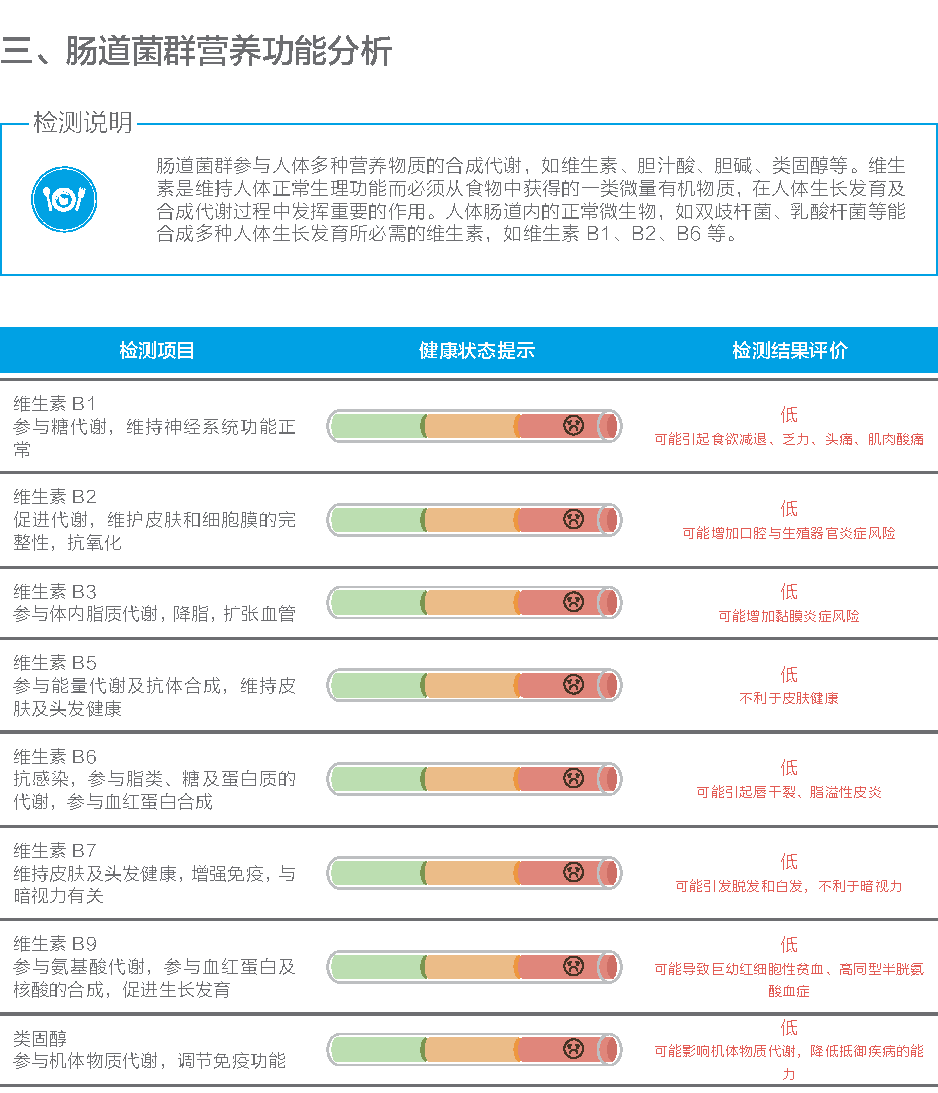
\includegraphics[width=\linewidth]{yingyanggongneng.pdf}
\asidebreak %
肠道菌群参与人体多种营养物质的合成代谢,如维生素、胆汁酸、胆碱、类固醇等。维生素是维持人体正常生理功能而必须从食物中获得的一类微量有机物质,在人体生长发育及合成代谢过程中发挥重要的作用。人体肠道内的正常微生物,如双歧杆菌、乳酸杆菌等能合成多种人体生长发育所必需的维生素,如维生素B1、B2、B6等。
\end{LRaside}

\vspace*{2mm}
%2.1 您的常见肠道菌含量
\vspace*{1.5mm}

%\begin{RCtable}{
%  rtab=1,
%  tabularx*={\arrayrulecolor{gray2}}%
%    {M{0.3\linewidth} M{0.31\linewidth}M{0.34\linewidth}}
%}
%\fuentecabecera{测试项目} & \fuentecabecera{健康状态提示} & \fuentecabecera{检测结果评价} \\[3pt]
%\bf{测试项目} & \bf{健康状态提示} & \bf{检测结果评价} \\[3pt]
%\end{RCtable}

\begin{tctabularx}{tabularx={m{4.8cm}<{\centering}m{5.2cm}<{\centering}m{4.55cm}<{\centering}}}
&&
\\[-6pt]
\cellcolor{topcolor} \raisebox{2.614pt}{\color{black00}\bf 检测项目} &
\cellcolor{topcolor} \raisebox{2.614pt}{\color{black00}\bf 健康状态提示} &
\cellcolor{topcolor} \raisebox{2.614pt}{\color{black00}\bf 检测结果评价}
\end{tctabularx}

\vspace*{-4.25mm}
\fontsize{8.8pt}{11pt}\selectfont
\arrayrulecolor{gray2}
\begin{longtable}{m{4.8cm}m{5.2cm}<{\centering}m{0cm}@{}m{4.61cm}<{\centering}}
\hline
\parbox[c]{\hsize}{\vskip7pt {\lantxh 维生素B1\\参与糖代谢,维持神经系统功能正常} \vskip7pt} & \parbox[c]{\hsize}{\vskip7pt\centerline{\raisebox{-1.5ex}{
\includegraphics[width=5cm,height=0.55cm]{bar.pdf}}}\vskip7pt}  &
\hspace*{-1.51cm}\raisebox{-0.45ex}{
\includegraphics{cry.pdf}}
 & \begin{minipage}{4.60cm}\begin{center}{{\color{red}\lantxh 低{\\ \bahao 可能引起食欲减退、乏力、头痛、肌肉酸痛}} }\end{center} \end{minipage} \\
% & \begin{minipage}{4.60cm}\begin{center}{{\color{red}\lantxh 低 \\ \bahao 可能引起食欲减退、乏力、头痛、肌肉酸痛} }\end{center} \end{minipage} \\
\hline
\parbox[c]{\hsize}{\vskip7pt {\lantxh 维生素B2\\促进代谢,维护皮肤和细胞膜的完整性,抗氧化} \vskip7pt} & \parbox[c]{\hsize}{\vskip7pt\centerline{\raisebox{-1.5ex}{
\includegraphics[width=5cm,height=0.55cm]{bar.pdf}}}\vskip7pt}  &
\hspace*{-1.51cm}\raisebox{-0.45ex}{
\includegraphics{cry.pdf}}
 & \begin{minipage}{4.60cm}\begin{center}{{\color{red}\lantxh 低{\\ \bahao 可能增加口腔与生殖器官炎症风险}} }\end{center} \end{minipage} \\
% & \begin{minipage}{4.60cm}\begin{center}{{\color{red}\lantxh 低 \\ \bahao 可能增加口腔与生殖器官炎症风险} }\end{center} \end{minipage} \\
\hline
\parbox[c]{\hsize}{\vskip7pt {\lantxh 维生素B3\\参与体内脂质代谢,降脂,扩张血管} \vskip7pt} & \parbox[c]{\hsize}{\vskip7pt\centerline{\raisebox{-1.5ex}{
\includegraphics[width=5cm,height=0.55cm]{bar.pdf}}}\vskip7pt}  &
\hspace*{-1.51cm}\raisebox{-0.45ex}{
\includegraphics{cry.pdf}}
 & \begin{minipage}{4.60cm}\begin{center}{{\color{red}\lantxh 低{\\ \bahao 可能增加黏膜炎症风险}} }\end{center} \end{minipage} \\
% & \begin{minipage}{4.60cm}\begin{center}{{\color{red}\lantxh 低 \\ \bahao 可能增加黏膜炎症风险} }\end{center} \end{minipage} \\
\hline
\parbox[c]{\hsize}{\vskip7pt {\lantxh 维生素B5\\参与能量代谢及抗体合成,维持皮肤及头发健康} \vskip7pt} & \parbox[c]{\hsize}{\vskip7pt\centerline{\raisebox{-1.5ex}{
\includegraphics[width=5cm,height=0.55cm]{bar.pdf}}}\vskip7pt}  &
\hspace*{-1.51cm}\raisebox{-0.45ex}{
\includegraphics{cry.pdf}}
 & \begin{minipage}{4.60cm}\begin{center}{{\color{red}\lantxh 低{\\ \bahao 不利于皮肤健康}} }\end{center} \end{minipage} \\
% & \begin{minipage}{4.60cm}\begin{center}{{\color{red}\lantxh 低 \\ \bahao 不利于皮肤健康} }\end{center} \end{minipage} \\
\hline
\parbox[c]{\hsize}{\vskip7pt {\lantxh 维生素B6\\抗感染,参与脂类、糖及蛋白质的代谢,参与血红蛋白合成} \vskip7pt} & \parbox[c]{\hsize}{\vskip7pt\centerline{\raisebox{-1.5ex}{
\includegraphics[width=5cm,height=0.55cm]{bar.pdf}}}\vskip7pt}  &
\hspace*{-1.51cm}\raisebox{-0.45ex}{
\includegraphics{cry.pdf}}
 & \begin{minipage}{4.60cm}\begin{center}{{\color{red}\lantxh 低{\\ \bahao 可能引起唇干裂、脂溢性皮炎}} }\end{center} \end{minipage} \\
% & \begin{minipage}{4.60cm}\begin{center}{{\color{red}\lantxh 低 \\ \bahao 可能引起唇干裂、脂溢性皮炎} }\end{center} \end{minipage} \\
\hline
\parbox[c]{\hsize}{\vskip7pt {\lantxh 维生素B7\\维持皮肤及头发健康,增强免疫,与暗视力有关} \vskip7pt} & \parbox[c]{\hsize}{\vskip7pt\centerline{\raisebox{-1.5ex}{
\includegraphics[width=5cm,height=0.55cm]{bar.pdf}}}\vskip7pt}  &
\hspace*{-1.51cm}\raisebox{-0.45ex}{
\includegraphics{cry.pdf}}
 & \begin{minipage}{4.60cm}\begin{center}{{\color{red}\lantxh 低{\\ \bahao 可能引发脱发和白发,不利于暗视力}} }\end{center} \end{minipage} \\
% & \begin{minipage}{4.60cm}\begin{center}{{\color{red}\lantxh 低 \\ \bahao 可能引发脱发和白发,不利于暗视力} }\end{center} \end{minipage} \\
\hline
\parbox[c]{\hsize}{\vskip7pt {\lantxh 维生素B9\\参与氨基酸代谢,参与血红蛋白及核酸的合成,促进生长发育} \vskip7pt} & \parbox[c]{\hsize}{\vskip7pt\centerline{\raisebox{-1.5ex}{
\includegraphics[width=5cm,height=0.55cm]{bar.pdf}}}\vskip7pt}  &
\hspace*{-1.51cm}\raisebox{-0.45ex}{
\includegraphics{cry.pdf}}
 & \begin{minipage}{4.60cm}\begin{center}{{\color{red}\lantxh 低{\\ \bahao 可能导致巨幼红细胞性贫血、高同型半胱氨酸血症}} }\end{center} \end{minipage} \\
% & \begin{minipage}{4.60cm}\begin{center}{{\color{red}\lantxh 低 \\ \bahao 可能导致巨幼红细胞性贫血、高同型半胱氨酸血症} }\end{center} \end{minipage} \\
\hline
\parbox[c]{\hsize}{\vskip7pt {\lantxh 类固醇\\参与机体物质代谢,调节免疫功能} \vskip7pt} & \parbox[c]{\hsize}{\vskip7pt\centerline{\raisebox{-1.5ex}{
\includegraphics[width=5cm,height=0.55cm]{bar.pdf}}}\vskip7pt}  &
\hspace*{-1.51cm}\raisebox{-0.45ex}{
\includegraphics{cry.pdf}}
 & \begin{minipage}{4.60cm}\begin{center}{{\color{red}\lantxh 低{\\ \bahao 可能影响机体物质代谢,降低抵御疾病的能力}} }\end{center} \end{minipage} \\
% & \begin{minipage}{4.60cm}\begin{center}{{\color{red}\lantxh 低 \\ \bahao 可能影响机体物质代谢,降低抵御疾病的能力} }\end{center} \end{minipage} \\
\hline
\parbox[c]{\hsize}{\vskip7pt {\lantxh 胆碱\\肠道细菌降解胆碱会生成TMAO,TMAO会增加心血管疾病风险} \vskip7pt} & \parbox[c]{\hsize}{\vskip7pt\centerline{\raisebox{-1.5ex}{
\includegraphics[width=5cm,height=0.55cm]{bar.pdf}}}\vskip7pt}  &
\hspace*{-4.83cm}\raisebox{-0.45ex}{
\includegraphics{smile.pdf}}
 & \begin{minipage}{4.60cm}\begin{center}{{\lantxh 低{}} }\end{center} \end{minipage} \\
% & \begin{minipage}{4.60cm}\begin{center}{{\lantxh 低 \\ \bahao -} }\end{center} \end{minipage} \\
\hline
\parbox[c]{\hsize}{\vskip7pt {\lantxh 辅酶Q\\激活细胞呼吸代谢,抗氧化,增强免疫力} \vskip7pt} & \parbox[c]{\hsize}{\vskip7pt\centerline{\raisebox{-1.5ex}{
\includegraphics[width=5cm,height=0.55cm]{bar.pdf}}}\vskip7pt}  &
\hspace*{-1.51cm}\raisebox{-0.45ex}{
\includegraphics{cry.pdf}}
 & \begin{minipage}{4.60cm}\begin{center}{{\color{red}\lantxh 低{\\ \bahao 可能降低免疫力及抗衰老能力}} }\end{center} \end{minipage} \\
% & \begin{minipage}{4.60cm}\begin{center}{{\color{red}\lantxh 低 \\ \bahao 可能降低免疫力及抗衰老能力} }\end{center} \end{minipage} \\
\hline
\parbox[c]{\hsize}{\vskip7pt {\lantxh 胆汁酸\\促进食物中脂类和脂溶性维生素的吸收} \vskip7pt} & \parbox[c]{\hsize}{\vskip7pt\centerline{\raisebox{-1.5ex}{
\includegraphics[width=5cm,height=0.55cm]{bar.pdf}}}\vskip7pt}  &
\hspace*{-1.51cm}\raisebox{-0.45ex}{
\includegraphics{cry.pdf}}
 & \begin{minipage}{4.60cm}\begin{center}{{\color{red}\lantxh 低{\\ \bahao 不利于摄取食物中的脂类与脂溶性维生素}} }\end{center} \end{minipage} \\
% & \begin{minipage}{4.60cm}\begin{center}{{\color{red}\lantxh 低 \\ \bahao 不利于摄取食物中的脂类与脂溶性维生素} }\end{center} \end{minipage} \\
\hline
\multicolumn{3}{l}{}\\
\multicolumn{3}{l}{
\includegraphics[scale=1]{greencircle.pdf} {\fontsize{9.3pt}{11pt}\selectfont \bf 绿色表示健康}   
\includegraphics[scale=1]{orangecircle.pdf}  {\fontsize{9.3pt}{11pt}\selectfont \bf 橙色表示需要关注}  
\includegraphics[scale=1]{redcircle.pdf} {\fontsize{9.3pt}{11pt}\selectfont \bf 红色表示有风险}}
\end{longtable}

\vspace*{1mm}
\fontsize{9.3pt}{11pt}\selectfont
\begin{LRaside}[.8]{结果分析}
\noindent

\includegraphics[width=\linewidth]{result_yingyanggongneng.pdf}
\asidebreak %
综合您的检测结果,您肠道内参与维生素B1、维生素B2、维生素B3、维生素B5、维生素B6等代谢的菌群含量异常,可能增加头痛、肌肉酸痛、口腔炎症等的风险,不利于皮肤健康、机体物质代谢、抗衰老等。建议您持续监测肠道健康。
\end{LRaside}

\end{document}

